\documentclass{article}
%Seitenränder
\usepackage{geometry}
\geometry{a4paper, left=30mm, right=30mm, top=25mm, bottom=25mm} 

%Encoding:
\usepackage{t1enc}
\usepackage[utf8]{inputenc}

%Mathematische Formeln:
\usepackage{amsmath}
\usepackage{amsfonts}
\usepackage{amssymb}
\usepackage{mathtools} %Erweitert das amsmath package
\usepackage{yhmath} %Erweiterte Schriftarten in Mathe-Umgebungen

\usepackage{graphicx}
\usepackage{framed}
% for \Yleft \Yright
\usepackage{stmaryrd}
\usepackage{xcolor} %Text und Grafiken farbig gestalten
\usepackage{multicol} %Mehrspaltiger Text

\usepackage{hyperref} %Verwandelt u.a. interne links in klickbare Verweise
\usepackage[shortlabels]{enumitem} %itemize, enumerate, description individuell anpassen
\usepackage{float} %Grafiken schöner einfügen
\usepackage{wrapfig} %Von Text umflossene Grafiken einfügen
\usepackage{tikz} %Automaten, Graphen, ... mit LaTeX darstellen
\usetikzlibrary{arrows,shapes,automata,petri,backgrounds,calc,intersections}

\usepackage{todonotes}
\usepackage[toc]{appendix}


% Titel in Kopfzeilen
\usepackage{fancyhdr}
\pagestyle{fancy}
\setlength{\headheight}{20pt}


% Format der Autorenkürzel definieren
\newcommand{\initials}[1]{\small{\textit{(#1)}} \normalsize}

%----------------------------------------------
% Hier euren Titel eintragen
\title{Implementing a CSP Solver\\\small{Lecture Hybrid Systems, summer '19}}
% Hier eure(n) Namen eintragen
\author{Patrick Burke and Lynn Liebert}

%Kopfzeile anpassen:
\fancyhead[R]{CSP Solver} %Hier Dokument-Titel eintragen (erscheint im Header). Falls eigentlicher Titel zu lang, hier Kurztitel einfügen!
\fancyhead[L]{P. Burke, L. Liebert} %Auch hier ggf. Kurzversionen der Namen, falls Header zu voll wird.

%Damit werden euer Titel und der Autor intern definiert (hier müsst ihr nichts ändern)
\hypersetup{
	pdftitle={\@title},
	pdfauthor={\@author}
}


%Beginn des eigentlichen Dokumentes:
%----------------------------------------------
\begin{document}
\maketitle %Setzt automatisch Titel, Autoren und Datum

\listoftodos

\begin{abstract}
\todo[inline]{ABSTRACT}
\end{abstract}

\tableofcontents
\newpage

This report was created by Patrick Burke and Lynn Liebert, in equal parts and on their own \textbf{AND STUFF}.
\todo[inline]{u know, write this}

\todo[inline]{Table who did wwhat}

\todo[inline]{Signature lines here}

\newpage
\section{Introduction}

\emph{Constraint satisfaction problems} model problems in many areas in science and industry.
A \emph{CSP} is modelled with a set of variables, each one having it's own domain, as well as constraints which describe the relationships between the variables.~\cite{MF19}

The domains are not necessarily bounded or unbounded, finite or infinite.
But in this task, only simplified CSPs are considered, they are bounded as well as finite.~\cite{MF19}
Because the task only considers simple CSPs, we use the terms ``CSP'' and ``simple CSP'' interchangeably.

This report uses the same definitions as the task description.

\subsection{Task Description}

The task was to write a tool which gets as input a single CSP in form of a plaintext file.
After receiving the input, the program is supposed to find out of there exists a solution for the given CSP and if so state on possible solution.

Two algorithms $\mathcal{A}$ and $\mathcal{B}$ were given in the task description, which are capable of determining if a CSP is satisfiable and give a solution if so.

We won't reiterate on the algorithms directly here, since they can be found in the task description.
However, we will briefly describe our implementation of these algorithms in section~\ref{?}.

\subsection{Why does proposition 1 hold?}\label{ssec:prop1}

\begin{enumerate}[(a)]
\item Why does proposition 1 hold? How can a solution be extracted from $\rho$? Give a comprehensible explanation. (A formal proof is not necessary.)
\end{enumerate}
Let's recall proposition 1 from~\cite{MF19}:

\paragraph{Proposition 1}
\emph{Let $\rho$ be an interval valuation.}
\emph{Then, if all simple constraints of a CSP $\mathcal{P}$ are satisfied by $\rho$ then there exists a (point) solution of $\mathcal{P}$ and, hence, $\mathcal{P}$ is satisfiable.}

%\paragraph{}
%Or informally: If we find a $\rho$ which satisfies all constraints $c \in C$, there exists a solution for the corresponding CSP.

\paragraph{}
An interval valuation is a mapping from a variable $x_i \in X$ to a non-empty interval $\rho(x_i)$ with $p(x_i) \subseteq D_i \subset \mathbb{Z}$.
Per definition 1, a solution $A$ to a CSP $\mathcal{P}$ is an n-tuple $A = \langle a_1, ..., a_n \rangle$ with (1) $a_i \in D_i$, s.t. (2) all constraints $c \in C$ are satisfied.~\cite{MF19}

Let $\rho$ be an interval valuation of a CSP $\mathcal{P}$ which satisfies all constraints $c \in C$.
Using the above definition of solutions of a CSP and interval valuations, we can see that $\forall a_i \in A: a_i \in \rho(x_i) \subseteq D_i$, hence we can pick a single value $a_i$ from each $\rho(x_i)$ to extract a solution $A$.
We know $A$ is then a solution, because both properties of a solution hold:

\begin{enumerate}[(1)]
    \item $\forall a_i \in A: a_i \in D_i$, and
    \item $A$ satisfies all constraints $c \in C$, because $\rho$ already does.
\end{enumerate}

\subsection{Soundness and Completeness of $\mathcal{A}$}
\begin{enumerate}[(b)]
\item Is algorithm $\mathcal{A}$ sound and complete, i.e. does $\mathcal{A}$ stop on each simple CSP with the correct result? Give reasons for your answer.
\end{enumerate}

Algorithm $\mathcal{P}$ is both sound and complete, because it traverses the search space in a complete manner and only returns correct results.
To explain this, we will use a tree-like structure as the search space and argue that the algorithm traverses this tree in a way that allows it to always stop with the correct result.

\paragraph{}
\todo{Draw search space}
Fig.~\ref{?} shows the search space as a tree.
Each node represents an interval valuation, with the root being the initial interval valuation and the children of each node being created as result of step 3 of the algorithm.
The algorithm dictates that $\rho_{i} \cup \rho_{ii} = \rho$ and $\rho_{i} \cap \rho_{ii} = \emptyset$.
Which is important, because otherwise parts of the variable intervals would be missing from, or occur more than once in the search space.

%In the tree, all solutions are in the leaves.
%The search space, and hence the tree, is big for a CSP with sufficiently many constraints, thus it's not feasible to build the whole tree to get to all solutions.
%\todo{Glaube ich jedenfalls, muss noch mal geprüft werden...}
%Thus, a depth-first search is done in this tree.
%If an interval valuation under which all constraints are true is found, the algorithm stops immediately with \emph{CSP $\mathcal{P}$ is satisfiable}.

\begin{lemma}\label{lemma:false-branches}
    %\todo{Either proof this or use something different than a lemma}
    Once an interval valuation $\rho$ is found which falsifies a single constraint, the entire branch rooting in that interval valuation can be ignored by the search for a result.
    It is impossible for the truth value to change by further exploring this branch, because the condition $max \rho(x) < min \rho(y) + k$ for each false simple bound stays false. 
\end{lemma}


\paragraph{Proof}

Let $\rho$ be in interval valuation under which at least one constraint is false, and have false simple bounds have the form $x \geq y + k$.

Were the algorithm $\mathcal{A}$ to execute the decision step when a constraint is false under the current interval valuation, only the following cases could occur:

Let $x \in X$ be a variable that is part of at least one of the false simple bounds.
Let $\rho'(x)$ and $\rho''(x)$ be interval valuations created from $\rho(x)$ according to step 3 of algorithm $\mathcal{A}$.
We know that $\max \rho'(x), \max \rho''(x) \leq \max \rho(x)$ holds, because the algorithm dictates that $\rho'(x) \cup \rho''(x) = \rho(x)$.
Thus, $\max \rho(x) < \min \rho(y) + k$ still holds for all simple bounds that $x$ is part of, which means their truth value stays unchanged.

Let $y \in X$, $\rho(y)$, $\rho'(y)$ and $\rho''(y)$ be a created analogous to before.
We know that $\min \rho'(y), \min \rho''(y) \geq \min \rho(y)$ holds, because the algorithm dictates that $\rho'(y) \cup \rho''(y) = \rho(y)$.
Thus, $\max \rho(x) < \min \rho(y) + k$ still holds for all simple bounds that $y$ is part of, which means their truth value stays unchanged.

If the interval valuation of a variable which is not part of any of the false simple bounds is split, the truth values of these simple bounds are obviously not going to change. $k$ cannot change. $\square$


%\paragraph{}
%Informally, a simple bound being inconclusive arrises from the interval valuations being too big.
%The algorithm reduces the size of the interval valuations by some means (for example by splitting the interval of a variable in half) each time step 3 is executed.
%The further the interval valuations are reduced, the nearer we get to a result, which can be either that the formula is satisfiable or not.
%For the figure this means that the solutions, if there're any, are found nearer to the bottom of that tree (if drawn the way as seen in fig.~\ref{?}).

\paragraph{}
\todo{Nodes in einem tree? Das klingt falsch...}
The algorithm traverses the search tree by asserting the interval valuations which are represented as nodes in the tree.
Whenever such an interval valuation is asserted, all possible cases are handled by the algorithm:

\begin{itemize}
    \item
        \textbf{All constraints are true.}
        In this case, the algorithm stops correctly with \emph{CSP $\mathcal{P}$ is satisfiable} because it found either a point solution or a set of solutions.
    
    \item
        \textbf{At least one constraint is false.}
        Because of Lemma~\ref{lemma:false-branches} we know that this branch of the search space is a dead-end.
        In this case, the algorithm backtracks to a previously created but unused interval valuation to explore the branch of the search space that roots there.
        If there's no such backtrack alternative, it means there are no branches left to explore, thus the algorithm stops correctly with \emph{CSP $\mathcal{P}$ is unsatisfiable}.
    \item
        \textbf{Neither of the two.}
        In this case there's no way to tell if the CSP is satisfiable or not.
        The algorithm opens up two new branches in the search tree in step 3, stores one as a backtrack alternative and continues the search in the other one.
\end{itemize}

\paragraph{}
\todo{Das stimmt doch, oder?}
As shown in section~\ref{ssec:prop1}, if a CSP $\mathcal{P}$ is satisfiable, each $\rho$ under which none of the constraints $c \in C$ are false contains a solution.
Together with the fact that the algorithm traverses the branches of search tree which can contain a solution shows that the algorithm will find the solution if one is present.
And if there're no branches left to explore, stop the search by saying that $\mathcal{P}$ is unsatisfiable.



%Der Algorithmus durchsucht alle Äste des Suchbaums die eine Lösung enthalten können, bis eine Lösung gefunden wurde.
%Weil der Suchbaum alle Lösungen enthält, ist der Algorithmus vollständig.
%Und weil der Algorithmus nur mit satisfiable anhält, wenn alle Constraints wahr sind, ist er auch sound.


%Each $c \in C$ can be in one of three separate states:
%
%\begin{enumerate}
%    \item \texttt{true}
%    \item \texttt{false}
%    \item \texttt{inconclusive}
%\end{enumerate}
%
%From this we can conclude, that, at all times, these seven possibilities of combinations of truth values of all $c \in C$ can occur:
%
%\begin{enumerate}
%    \item All true
%    \item All false
%    \item All inconclusive
%    \item Some true, some false
%    \item Some true, some inconclusive
%    \item Some false, some inconclusive
%    \item Some true, some false, some inconclusive
%\end{enumerate}
%
%The only times the truth values of the constraints can change at all are when the interval valuation changes, this can happen in steps 2 and 3.
%Whenever this happens, the algorithm immediately goes to step 1.
%
%Step 1 correctly stops with $\mathcal{P}$ \emph{is satisfiable} when all $c \in C$ are true.
%
%The algorithm stops either in step 1 or step 2.
%
%
%Steps 1 and 3 behave the same way, no matter how many steps the algorithm has made up to the current point of execution (there is no ``state'' except for $\rho$).

%\subsubsection{Soundness}
%
%By contradiction.
%
%Let's assume a satisfiable CSP $\mathcal{P}$.
%Let's further assume that the Algorithm $\mathcal{A}$ applied to that CSP stops with the answer \emph{$\mathcal{P}$ is unsatisfiable}.
%
%For this to happen, the algorithm must have come across the step 2 and discover that there are no previously unused decision steps, because this is the only way the algorithm stops with ``unsatisfiable''.
%
%This can only happen when the cases 2, 4, 6 or 7 occur, and step 3 was executed as many times as step 2.
%
%
%\subsubsection{sldkf;dkfhlskjh}
%
%Im ersten Schritt diese Faelle:
%
%1. Alle True ->
%stoppt korrekt mit satisfiable
%
%2. Alle oder wenigstens einer False -> 
%Schritt 2
%
%3. Einige oder keine true, einige oder alle inkonklusiv ->
%Schritt 3
%
%
%Im zweiten Schritt (backtracking):
%
%1. Decision Level = 0 -> stoppt, mit unsatisfiable (z.b. der Fall direkt bei der 1. Iteration wenigstens ein constraint false ist)
%
%2. Decision Level > 0 -> 
%Verwende neues $\rho$, dann Schritt 1
%
%
%Im dritten Schritt:
%
%1. Es muss hier immer eine Variable geben, dessen $\rho$ wir aufteilen können.
%Das ist auch der Fall, denn wenn in einem simple bound $x \geq y + k$ $|\rho(x)| = |\rho(y)| = 1$ gilt, ist dieses entweder true oder false, und somit nicht inkonklusiv. Wenn dies für alle Variablen gilt, sind auch alle SImple bounds entweder true oder false, was bedeuten würde das wir gar nicht in diesem Schritt landen würden.

\subsection{NP-completeness}

\begin{enumerate}[(c)]
\item Why is constraint solving NP-complete for the given type of constraints formulae?
\end{enumerate}

Because using the following rules, a simple CSP problem can be created from arbitrary boolean SAT problems, which are known to be NP-complete.

\paragraph{}
Let $F_{sat}$ be a formula of a boolean SAT problem, with $n$ clauses and $m$ literals.
Let $F_{csp}$ be a formula of a CSP as defined in def.~3 from~\cite{MF19}, where $F_{csp} = k_1 \wedge\, k_2 \wedge\, ...$ and $k_{*}$ be constraints as defined in def.~2 from~\cite{MF19}.
Let $c_j$ be a clause, $l_i$ be a literal in $F_{sat}$, with $j \in \{1,..., n\}$ and $i \in \{1, ..., m\}$.
$z \in [0, 0]$ is an integer variable representing the value 0, and $k \in \mathbb{Z}$.

\begin{enumerate}
    \item For every literal $l_i$ in $F_{sat}$ a variable $x_i$ in $F_{csp}$ is created, with $D_i = [0,1]$.
    \item For every clause $c_j$ in $F_{sat}$:
    \begin{enumerate}
        \item A variable $y_j$ in $F_{csp}$ is created, with $D_j = [0,1]$.
            \item For every literal $l_i$ in that clause, a simple bound of the form $y_j \geq x_i + k$ is created, with
            \begin{enumerate}
                \item $k=0$ when the literal in $F_{sat}$ is \textbf{not} negated
                \item $k=1$ when the literal in $F_{sat}$ is negated
            \end{enumerate}
    \end{enumerate}
    \item A constraint is created in $F_{csp}$, which for each $y_j$ contains a simple bound of the form $y_j \geq z + 1$.
\end{enumerate}

\paragraph{}
The following formulae show a very simple boolean SAT formula and it's CSP counterpart, constructed by the aforementioned rules:

\begin{align*}
    F_{sat} =\, &x_1\\
    F_{csp} =\, &(y_1 \geq x_1 + 0) \wedge (y_1 \geq z + 1)
\end{align*}

\paragraph{}
Here is a more complex example, with colouring to aid in identifying related parts:

\begin{align*}
    F_{sat} =\,      &\textcolor{blue}{ (\neg x_1 \vee x_2 \vee x_3) }\\
            \wedge\, &\textcolor{red}{  (x_1 \vee \neg x_2)          }\\
    \\
    F_{csp} =\,      &\textcolor{blue}{ (y_1 \geq x_1 + 1 \vee y_2 \geq x_2 + 0 \vee y_3 \geq x_3 + 0) }\\
            \wedge\, &\textcolor{red}{  (y_4 \geq x_1 + 0 \vee y_5 \geq x_2 + 1)                       }\\
            \wedge\, &\textcolor{blue}{ (y_1 \geq z + 1 \vee y_2 \geq z + 1 \vee y_3 \geq z + 1)       }\\
            \wedge\, &\textcolor{red}{  (y_4 \geq z + 1 \vee y_5 \geq z + 1)                           }
\end{align*}

If a solution of a CSP created this way is found, that solution also solves the according boolean SAT problem.
And because boolean SAT problems are known to be NP-complete, simple CSPs as defined in def.~1 from~\cite{MF19} are also.

\subsection{Algorithm~$\mathcal{A}$ with real-valued bounds}

\begin{enumerate}[(d)]
    \item Assume that we generalize the definition of a simple CSP s.t. the domains of the variables are (possibly) infinite, but still bounded, e.g. intervals over the reals, and simple bounds are of the form $x \sim y + r$ with $\sim \in {\geq , >}$ and $r \in R$. Let $\mathcal{P}$ be such a generalized simple CSP.
    \begin{enumerate}[i.]
        \item Does algorithm $\mathcal{A}$ work correctly on $\mathcal{P}$, i.e. is the result correct? If this is not the case, can $\mathcal{A}$ be adapted? Give reasons for your answer.
        \item Does algorithm $\mathcal{A}$ terminate on $\mathcal{P}$? If this is not the case, can $\mathcal{A}$ be adapted? Give reasons for your answer.
    \end{enumerate}
    Remark: we consider the algorithm here in theory and not its behavior on a resource limited machine.
\end{enumerate}

Using $\mathcal{A}$ on $\mathcal{P}$ should have no effect on the the algorithm being correct, as long as it terminates. Splitting intervals is easier than before, since one is no longer restricted to only picking whole numbers to split intervals at. We are looking at the algorithm in a theoretical way and without the restrictions of a resource-limited machine, determining if two numbers are equal should not be a problem either. 

If a constraint is considered inconclusive and the splitting of an interval is induced, the constraint may keep being inconclusive, despite the variable interval being split. This process can keep repeating, because the termination condition is only fulfilled, when the amount of elements in the chosen interval is lower than 1. For real numbers, this can not be true, since there are infinite numbers between every two numbers. In this case of repeated splitting of an interval without any effect on the constraint being inconclusive, the algorithm does not terminate.




\subsection{Decision Heuristics}

\begin{enumerate}[(e)]
    \item \textbf{Optional:} Think about possible decision heuristics: Which heuristics –in your opinion– for a variable choice, for interval splitting and interval deciding make sense in this framework and why?
\end{enumerate}

Only the intervals of variables which are contained in constraints that are inconclusive at the time of interval splitting should be split. Should a variable v1 be contained only in constrain c1, which is true at the time of the split, while constraint c2 is the one being inconclusive, splitting the interval of v1 has no impact on the truth value of the inconclusive constraint c2. The algorithm should therefore choose a different variable, one that is actually contained in c2.

\todo[inline]{Hier kann man noch schnell was hinschreiben, denke ich.}

\section{Erster Abschnitt \initials{M.M.}}
Nach den (Unter-) Kapitelüberschriften soll mit Hilfe von Initialen angegeben werden, wer diesen Abschnitt verfasst hat. Hierzu muss lediglich wie oben im Beispiel gesehen \initials{V.N.} (LaTeX-Code siehe .tex-Datei) hinter einer Kapitelüberschrift eingefügt werden (wobei hier V der Anfangsbuchstabe des Vornamens und N der Anfangsbuchstabe des Nachnamen ist). 
\subsection{Unterabschnitt 1 von Abschnitt 1 \initials{J.M.}}
Eine Aufzählung:
\begin{itemize}
    \item Aufzählungspunkt 1
    \item Aufzählungspunkt 2
	\begin{itemize}
	    \item Aufzählungen können 
	    \item auch verschachtelt werden!
	    \item ...
	\end{itemize}    
    \item Aufzählungspunkt 3
	\begin{enumerate}
	    \item Oder verschachtelt
	    \item \textbf{und} nummeriert!
	    \item ...
	\end{enumerate}
\end{itemize}
Eine andere Art der Aufzählung:
\begin{description}
    \item[Punkt 1: ] Beliebiger Text.
    \item[Punkt 2: ] Beliebiger anderer Text.
\end{description}

\subsection{Unterabschnitt 2 von Abschnitt 1 \initials{M.M.}}
Eine Tabelle:
\par\medskip %Ein mittlerer Absatz
\begin{tabular}{|l|p{4cm}|c|} %1. Spalte linksbündig, 2. Spalte 4cm breit, 3. Spalte zentriert
    \hline
    % Zeile 1:
    Zelle 0,0 & Zelle 0,1 & Zelle 0,2 \\ %Das & trennt die Zelleneinträge voneinander
    \hline
    % Zeile 2:
    Zelle 1,0 & Zelle 1,1 & Zelle 1,2 \\
    \hline
\end{tabular}
\par\smallskip

Mathematische Formel:
\begin{align*} % align zentriert die Formel automatisch
    x &= {\sum}_{i=0}^{n} \frac{y_i}{2} \\ %Durch &= stehen die Gleichheitszeichen untereinander
      &= \pi - 42
\end{align*}
Mathematische Formeln wie $x=x_1 +x_2$ können auch im Fließtext integriert werden. Quellen werden mit \cite{AB12} zitiert und tauchen dann in der Literaturliste auf.

\section{Zweiter Abschnitt \initials{M.M., J.M.}}
Grafiken oder Text können mit multicols nebeneinander arrangiert werden. Mit LaTeX TikZ können auch Graphen oder Automaten modelliert werden:

\begin{multicols}{2} % Multicols ermöglicht es zwei (oder mehr) Grafiken oder Textpassagen nebeneinander anzuordnen. 
Eine Grafik mit TikZ:
	    \begin{figure}[H]
		\centering
		\begin{tikzpicture}[, ->,>=stealth',shorten >=0pt,auto,node distance=3cm,
                semithick, scale=0.9, transform shape]
		\begin{scope}
			\node [state, fill=blue!20] (l0) [label=left:{$\{x\}$}]{$l_0$};
			\node [state, fill=blue!20] (l1) [right of=l0, label=right:{\textcolor{blue}{$10$}}]{$l_1$};
			\node [state, fill=blue!20] (l2) [below of=l0, label=below:{hallo}]{$l_2$};
			
		    	\path (l0) edge [bend left=00] node[xshift=+0.9cm, yshift=-0.46cm] {\parbox{3cm}{$y > 0 /$ \\ $y:=0$}} (l1)
			      (l1) edge [bend left=00] node {$x:=0$} (l2)
			      (l2) edge [bend left=00] node {$x:=y$} (l0);
		\end{scope}
		\end{tikzpicture}
		\caption{Bildunterschrift}
	    \end{figure}
\columnbreak
Eine andere Grafik mit TikZ:
	    \begin{figure}[H]
		\centering
		\begin{tikzpicture}[initial text=, ->,>=stealth',shorten >=0pt,auto,node distance=3cm,
                semithick, scale = 0.9, transform shape]
		\begin{scope}
			\node [state, initial] (r0) {$r_0$};
			\node [state, rectangle] (r1) [right of=r0]{$r_1$};
			\node [state] (r2) [below of=r0] {$r_2$};
			\node [state, accepting] (r3) [below of=r1] {$r_3$};
			
		    	\path (r0) edge [bend left=20] node {$x>10$} (r1)
			      (r1) edge [bend left=20, dashed] node {$x>20/x:=0$} (r0)
			      (r0) edge [dotted] node {\textcolor{red}{fail}} (r2)
			      (r1) edge node {$x\geq15$} (r3)
			      (r2) edge [loop right] (r2);
		\end{scope}
		\end{tikzpicture}
	    \end{figure}
\end{multicols}

Hier kommt nun viel Text. Hier kommt nun viel Text. Hier kommt nun viel Text. Hier kommt nun viel Text. Hier kommt nun viel Text. Hier kommt nun viel Text. Hier kommt nun viel Text. Hier kommt nun viel Text.
\par\smallskip

Hier kommt nun viel Text. Hier kommt nun viel Text. Hier kommt nun viel Text. Hier kommt nun viel Text. Hier kommt nun viel Text. Hier kommt nun viel Text. Hier kommt nun viel Text. Hier kommt nun viel Text. Hier kommt nun viel Text. Hier kommt nun viel Text.
\begin{wrapfigure}[12]{r}{4.5cm} %#1: Zeilenanzahl
    \includegraphics[width=4.3cm]{images/Ente}
    \caption{\small{Quelle: wikimedia}}
\end{wrapfigure}
Hier kommt nun viel Text. Hier kommt nun viel Text. Hier kommt nun viel Text. Hier kommt nun viel Text. Hier kommt nun viel Text. Hier kommt nun viel Text. Hier kommt nun viel Text. Hier kommt nun viel Text. Hier kommt nun viel Text. Hier kommt nun viel Text.  Hier kommt nun viel Text. Hier kommt nun viel Text. Hier kommt nun viel Text. Hier kommt nun viel Text. Hier kommt nun viel Text. Hier kommt nun viel Text. Hier kommt nun viel Text. Hier kommt nun viel Text. Hier kommt nun viel Text. Hier kommt nun viel Text. Hier kommt nun viel Text. Hier kommt nun viel Text. Hier kommt nun viel Text. Hier kommt nun viel Text. Hier kommt nun viel Text. Hier kommt nun viel Text. Hier kommt nun viel Text. Hier kommt nun viel Text. Hier kommt nun viel Text. Hier kommt nun viel Text. Hier kommt nun viel Text. Hier kommt nun viel Text. Hier kommt nun viel Text. Hier kommt nun viel Text. Hier kommt nun viel Text. Hier kommt nun viel Text. Hier kommt nun viel Text. Hier kommt nun viel Text. Hier kommt nun viel Text. Hier kommt nun viel Text.   Hier kommt nun viel Text.
\par\smallskip %Kleiner Absatz
Hier kommt nun viel Text. Hier kommt nun viel Text. Hier kommt nun viel Text. Hier kommt nun viel Text. Hier kommt nun viel Text. Hier kommt nun viel Text. Hier kommt nun viel Text. Hier kommt nun viel Text. Hier kommt nun viel Text. Hier kommt nun viel Text. Hier kommt nun viel Text. Hier kommt nun viel Text. Hier kommt nun viel Text.   Hier kommt nun viel Text. Hier kommt nun viel Text. Hier kommt nun viel Text. Hier kommt nun viel Text. Hier kommt nun viel Text. Hier kommt nun viel Text. Hier kommt nun viel Text. Hier kommt nun viel Text. Hier kommt nun viel Text. Hier kommt nun viel Text.   Hier kommt nun viel Text. Hier kommt nun viel Text. Hier kommt nun viel Text. Hier kommt nun viel Text. Hier kommt nun viel Text.   Hier kommt nun viel Text.
\par\bigskip %Großer Absatz

Damit die folgende Literaturliste angezeigt wird, müsst ihr eure Literatur in die bib.bib Datei eintragen und anschließend zunächst pdflatex ausführen, danach bibtex, danach wieder pdflatex.

\appendix
\section{Definitions}\label{sec:apx:definitions}
\todo[inline]{Put the definitions from task description here}


\paragraph{Definition 1 (CSP)}
Ein CSP ist ein Tripel $\mathcal{P} = \langle X, D, C \rangle$ mit:

\begin{itemize}
    \item $X = \langle x_1, ..., x_n \rangle$ ein n-Tupel von Variablen
    \item $D = \langle D_1, ..., D_n \rangle$ ein n-Tupel von Definitionsbereichen, sodass $x_i \in D_i, i \in \{1, ..., n\}$, und
    \item $C = \langle c_1, ..., c_t \rangle$ ein t-Tupel von Bedingungen.
\end{itemize}



\section{Sample CSPs and Output}

\section{Commented Source Code}

\todo[inline]{Keine Ahnung ob wir das tun sollten... Vielleicht den entscheidenen Teil oder so?}

\bibliographystyle{plain}
\bibliography{bib}

\end{document}
